\section{Задание}

\hspace*{5mm} Реализовать программу для построения графиков функции и плотности для следующих распределений:
\begin{itemize}
  \item равномерное распределение;
  \item нормальное распределение (вариант 3).
\end{itemize}


\section{Теоритическая часть}
\subsection{Равномерное распределение}

Плотность распределения представлена в формуле \ref{eq:uniform_pdf}.

\begin{equation}\label{eq:uniform_pdf}
  f_X(x) =
  \begin{cases}
    \dfrac{1}{b-a},  \hspace*{1cm} x \in [a,b] \\
    \quad 0,         \hspace*{1.4cm} x \notin [a, b] \\
  \end{cases}
\end{equation}

Функция распределения представлена в формуле \ref{eq:uniform_cdf}.

\begin{equation}\label{eq:uniform_cdf}
  F_X(x) =
  \begin{cases}
    \quad 0,         \hspace*{1.4cm} x < a \\
    \dfrac{x-a}{b-a},\hspace*{1cm} a \le x < b \\
    \quad 1,         \hspace*{1.4cm} x \geq b \\
  \end{cases}
\end{equation}

\subsection{Нормальное распределение}

Плотность распределения представлена в формуле \ref{eq:norm_pdf}.

\begin{equation}\label{eq:norm_pdf}
  f_X(x) = \dfrac{1}{\sigma \sqrt{2 \pi}} e^{-\dfrac{(x - \mu)^2}{2 \sigma^2}}
\end{equation}

Функция распределения представлена в формуле \ref{eq:norm_cdf}.

\begin{equation}\label{eq:norm_cdf}
  F (x) = \dfrac{1}{\sigma \sqrt{2\pi}} \int_{-\infty}^x e^{-\dfrac{(t- \mu)^2}{2 \sigma^2}} dt
\end{equation}
\pagebreak

\section{Результаты}
\subsection{Равномерное распределение}

\begin{figure}[h!]
  \centering
  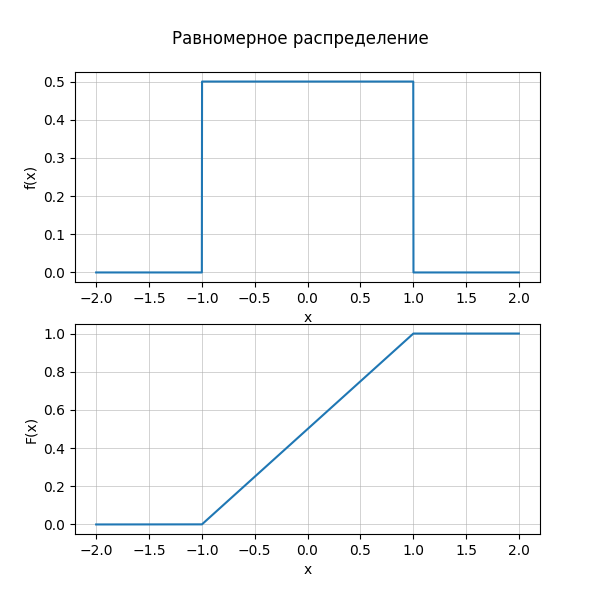
\includegraphics[scale=0.65]{1/uniform1}
  \caption{Равномерное распределение при a = -1, b = 1}
\end{figure}

\begin{figure}[h!]
  \centering
  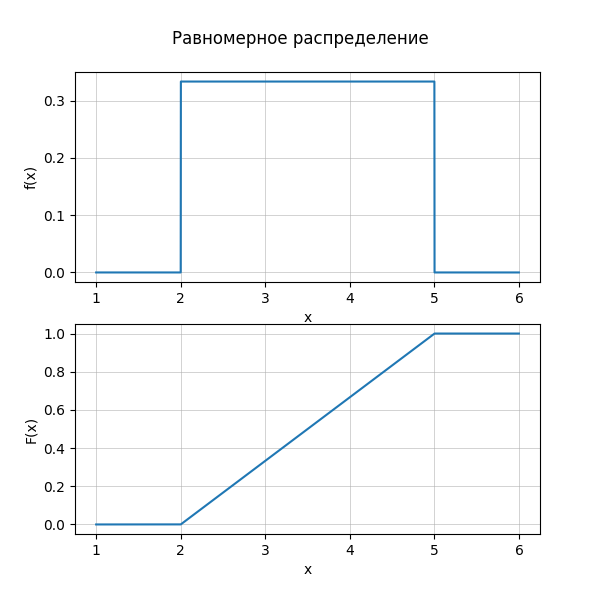
\includegraphics[scale=0.65]{1/uniform2}
  \caption{Равномерное распределение при a = 2, b = 5}
\end{figure}
\pagebreak

\subsection{Нормальное распределение}
\begin{figure}[h!]
  \centering
  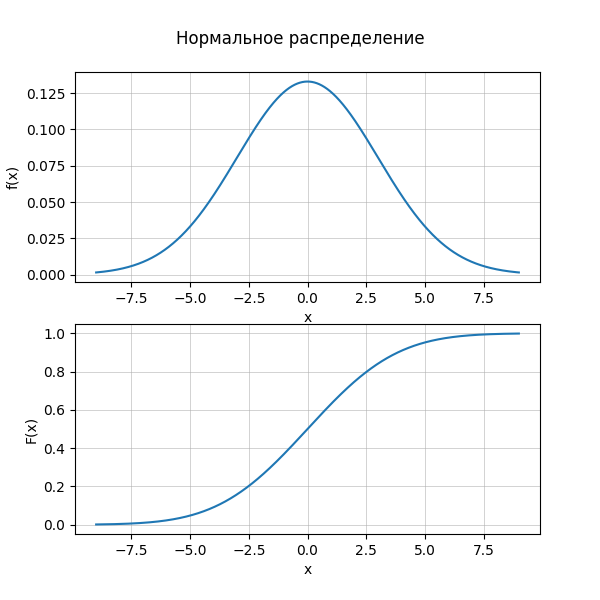
\includegraphics[scale=0.65]{1/norm1}
  \caption{Нормальное распределение при $\mu$ = 0, $\sigma$ = 3}
\end{figure}

\begin{figure}[h!]
  \centering
  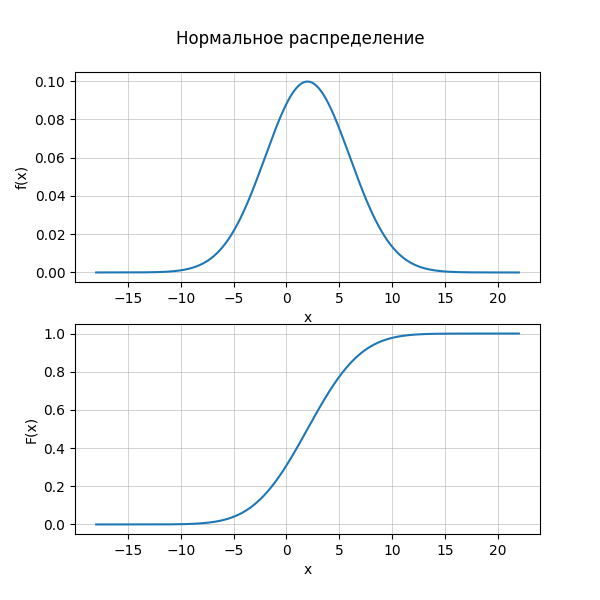
\includegraphics[scale=0.65]{1/norm2}
  \caption{Нормальное распределение при $\mu$ = 2, $\sigma$ = 4}
\end{figure}
\pagebreak

\section{Листинг кода}

\lstinputlisting[language=Python, caption=Программная реализация равномерного распределения и нормального распределения]{../1/main.py}
